\subsection{Preliminary Results}
\label{ss:results}

\begin{figure}[t]
  \center{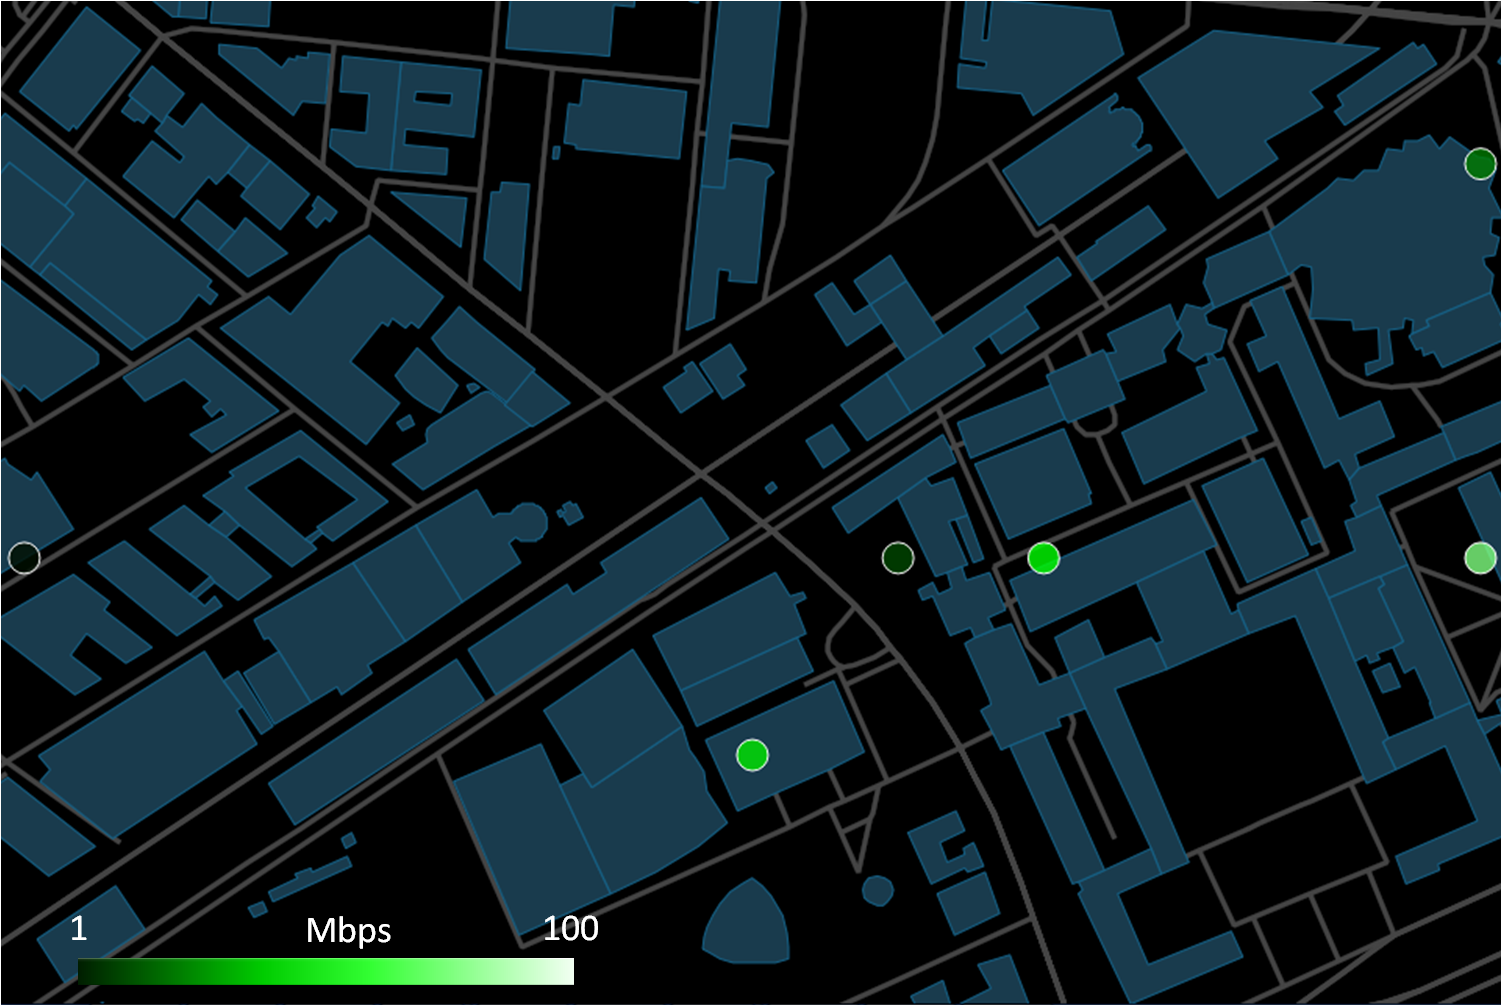
\includegraphics[width=85mm]{figures/bw.png}}
  \caption{
    The map of the WiFi/cellular network bandwidth.
  }
  \label{fig:bw}
\end{figure}

\begin{figure}[t]
  \center{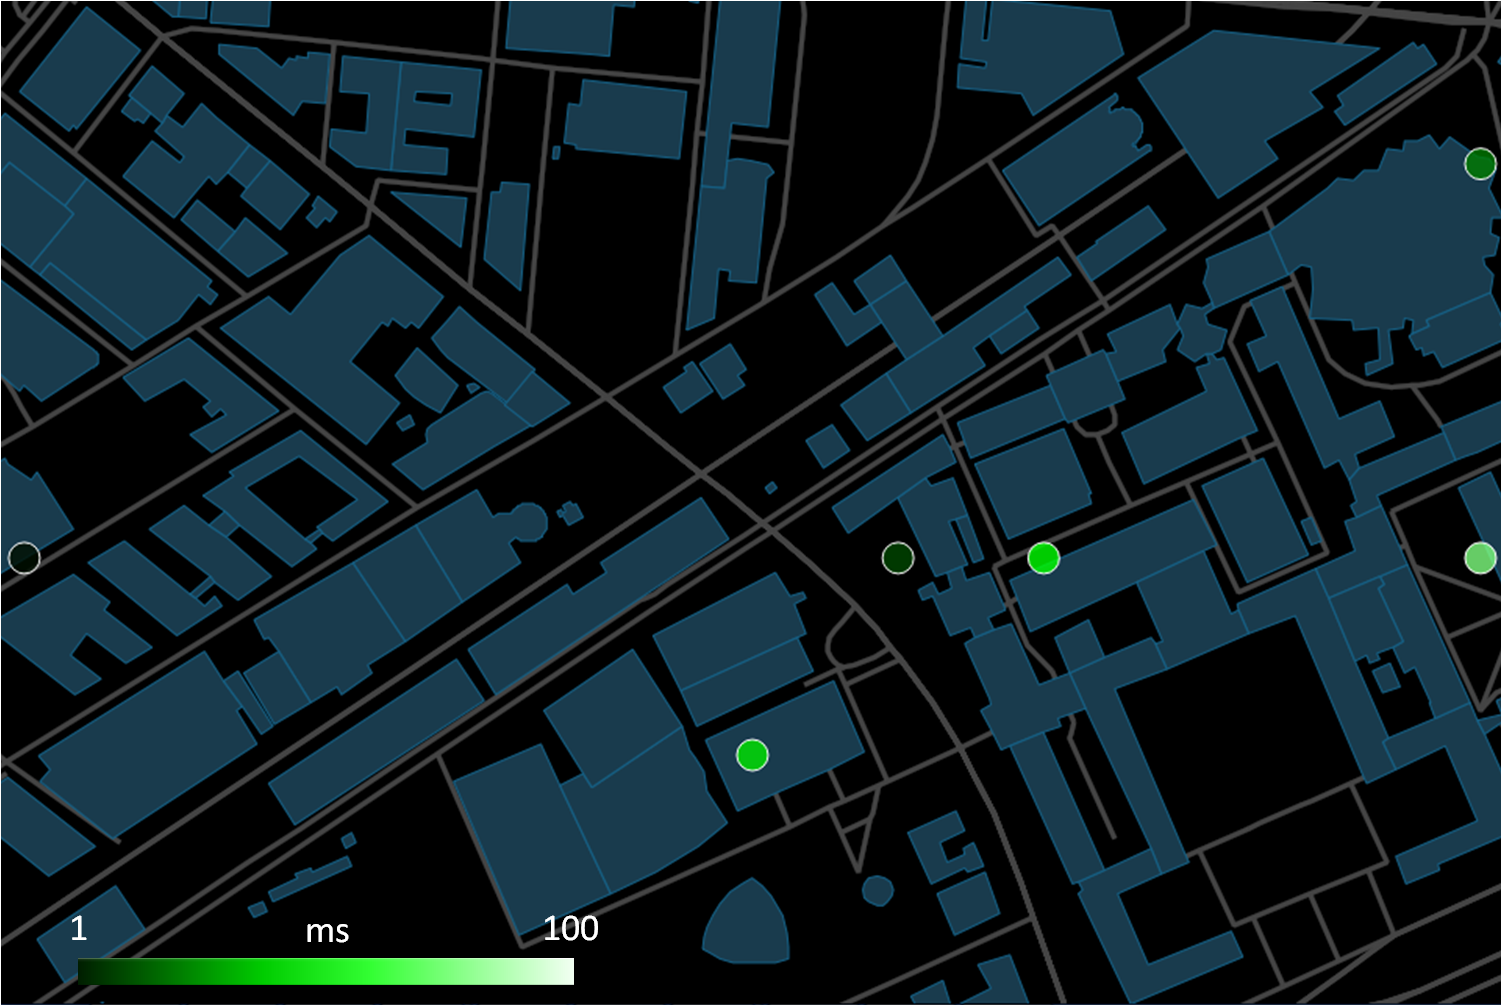
\includegraphics[width=85mm]{figures/rtt.png}}
  \caption{
    The map of the WiFi/cellular network average round-trip-time.
  }
  \label{fig:rtt}
\end{figure}

In this section, we present the map of several network performance
metrics based on the data we collected. This is one of the many possible 
applications that can be realized using \name{}'s data. 

We implemented an Android application using \name{}'s measurement 
library API and collected data around the MIT campus. 
All the measurements are uploaded and stored in the \name{} Server.
To visualize the network performance metrics on a map, we divide the map
into multiple grids, average all the values within a particular grid, and
plot the average value as a circle at the center of the grid. 

{\bfseries Bandwidth.}
Figure~\ref{fig:bw} shows the map of the WiFi/cellular network bandwidth.
As we mentioned in the introduction, wireless Internet connection performance 
varies greatly. The map clearly illustrates the spatial variation. The bandwidth
ranges from 1 to 90 Mbps within a small distance, and under the same administrative
domain (MIT's IS\&T). Therefore, a possible consequence is that we'll need to 
be able to handle hi-resolution data to produce an accurate map.

{\bfseries Average Round-Trip-Time.}
Figure~\ref{fig:rtt} presents the map of the WiFi/cellular network average
round-trip-time. We make two observations. First, the average RTT also 
varies with location (between 20 to 800 ms). Second, there is no clear 
correlation between the network bandwidth and average RTT. Places with a
higher bandwidth does imply a shorter RTT. 
